% We started doing 1-page reports, so some layout stuff will have to be
% changed.  When asked what it's supposed to look like, Weatherford said it's
% ``memo format'' with 2 graphs and a brief conclusion.

% I (Charles) assume that means there's an abstract, results (just graphs,
% probably), and a short description/analysis of the results; the sections will
% be changed accordingly.

\documentclass{article}
\usepackage{graphicx}
\usepackage{float}
\usepackage[acronym]{glossaries}
\usepackage{fullpage}
\usepackage{caption}
\usepackage{subcaption}

\loadglsentries{acronyms}
\makeglossaries

\begin{document}

\begin{tabular}{rl}
  \textbf{Lab 6:} & Separately Excited DC Motor \\
  \textbf{Performed:} & March 4, 2013 \\
  \textbf{Partners:} & Rawley Dent \\ & Charles Pittman \\
  \textbf{Instructor:} & Dr. Weatherford
\end{tabular}

%\setlength\parindent{0pt}

\section*{Abstract}

In this experiment, the operating characteristics of a separately excited dc motor were analyzed. 
This report highlights two parts: the investigation of the relationship between motor torque and 
armature current, and the investigation of dc motor saturation effects. The procedure to determine
the motor torque and armature current relationship consisted of increasing the dynanometer load torque
while keeping the voltage supply constant at 116.5-V. A set of data containing the load torque and 
the armature current were recorded and analyzed. The procedure to determine the dc motor saturation 
effects consisted of using the field control rheostat to increase the field current while keeping the 
armature current constant at 1.5-A. A set of data containing the output torque and field current were 
recorded and analyzed.

\section*{Results}

\begin{figure}[H]
  \centering
  \begin{subfigure}[b]{0.45\textwidth}
    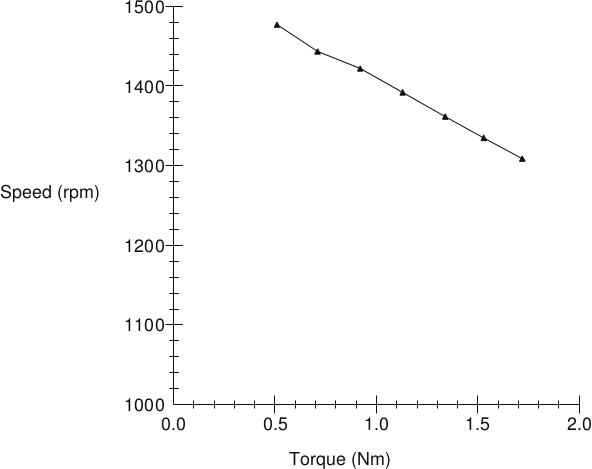
\includegraphics[width=\textwidth]{img/plot4}
    \caption{\textbf{DC Motor Speed vs. Torque}}
    \label{fig:plot4}
  \end{subfigure}~% The tilde is to keep them side-by-side
%
  \begin{subfigure}[b]{0.45\textwidth}
    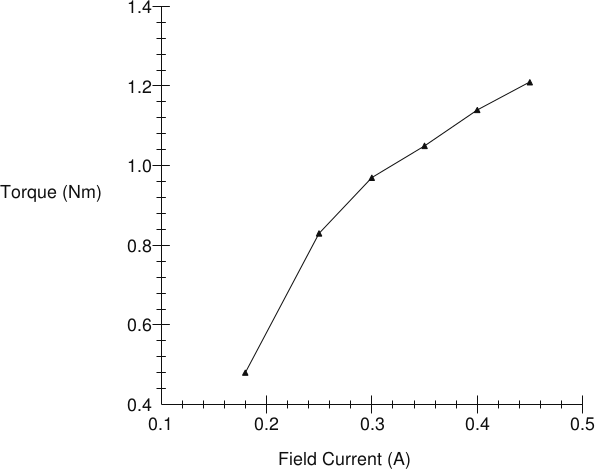
\includegraphics[width=\textwidth]{img/plot5}
    \caption{\textbf{DC Motor Torque vs. Field Current}}
    \label{fig:plot5}
  \end{subfigure}
\end{figure}

\section*{Conclusions}

In Figure~\ref{fig:plot4}, the linear relationship between dc motor speed $n_m$ and torque \tau is exemplified.
The dc motor was initially operating at approximately 1500 rpm. As the load torque was increased, the
dc motor experienced a decrease in speed. The armature current was also increasing while the load torque
was increasing, and thus the internal genearated voltage $E_A$ was decreased.

In Figure~\ref{fig:plot5}, the dc motor saturation effects are shown. This plot is similar to a dc motor
magnetization curve, where the field current is plotted against the internal voltage. Here, the field current was
plotted against the output torque. Since the torque in any real machine depends on the flux in the machine, 
and the internal voltage $E_A$ is directly proportional to the flux produced, the y-axis in Figure~\ref{fig:plot5}
can be represented by torque and not $E_A$ as in a dc machine magnetization curve. This plot shows that initially
a large increase in field current correlates to a sharp increase in output torque. Initially the dynamometer load
torque was set to its max value. Thus as the dc motor output torque nears this max dynamometer load torque, 
further increases in field current produce less and less increases in output torque.


\end{document}
